\chapter{Úvod}
\chapter{Přehled teorie}
\label{prehled}

V teto kapitole jsou popsaný teoretické základy Petřino sítí. Taky tato kapitola se soustředí na popis několika podtříd Petriho sítě, zejména na „vysokoúrovňové Petriho sítě“ a „Značkované Petriho Sítě“ a  včetně přehledu míst, kdě se tento modelovací prostředek používá, a hra významnou roli.

Dalším účelem této kapitoly je seznámení čtenáře s matematickými popisy Petriho síti a grafy Petriho sítí, které jsou nezbytné pro porozumění principu prací simulátoru.

Do obsahu patří popis protokolu MQTT \ref{subsec:mqtt-proto}, na kterém je založena externí komunikace simulátoru \ref{subsec:mqtt_impl}.

Taky se tady zmíní o simulační teorii, zaměřené na simulaci Petriho síti v reálném čase. Vyjasní se pojem distribuovaných systému \ref{subsec:distr_system}, HWIL \ref{subsec:hwil} a jejích vztah z Petriho sítěmi.

\subsection{Petriho sítě}
V současné době se Petriho sítě často používají jako modelovací prostředek pro modelovaní chovaní systému, za účelem pochopení jeho slabších stránek, ještě než se system nasadí do provozu. Vyplňuje, tím pádem, díru mezi slovním popisem, návrhem, takovými modelovacími prostředky jako \href{https://en.wikipedia.org/wiki/Unified_Modeling_Language}{UML} a skutečnou implementací nějakého projektu. Použití Petriho síti pro účel modelování je velice vhodné, jen velmi málo modelovacích prostředku dokáže popsat ne jenom system jako celek, ale i zjistit slabší stránky jeho implementace, ještě před implementační fází. Stejně tak platí i pro testovací fází -- některé chyby se dá objevit jenom po implementací, když to Petriho sítě částečně řeší tento problém ještě ve fází navrchu.

\paragraph{Definice}

Petriho síť ($PN$) se sestavuje ze čtyřce prvku, $PN = \left(P, T, I, O\right)$ kde:
  \begin{itemize}
    \item $P = \left\{p_1, p_2, \cdots , p_n\right\}$ je konečná množina míst, $n >= 0$; \\
    \item $T = \left\{t_1, t_2, \cdots , t_m\right\}$ je konečná množina přechodů, $m >= 0$; \\
    \item $I = T \rightarrow P^\infty$ je vstupní funkce, propojující přechody s množinou vstupních míst; \\
    \item $O = P \rightarrow T^\infty$ je výstupní funkce, propojující výstupní místa s množinou přechodů; \\
  \end{itemize}
P $\vee$ T = $\varnothing$, P $\wedge$ T != $\varnothing$.

\section{Typy Petriho sítě}

\subsection{Značkované Petriho sítě}
Značkované petriho seti (ZPS) zavadí takový pojem jako značka nebo \uv{token}. Značka je základní prvek v ZPS, umožnující její vykonávaní. Vykonávaní se provádí provedením přechodu, během kterého se vymaže odpovídající počet značek ze množiny vstupních míst, a do výstupních míst se potřebný počet značek vloží. Tato operace se muže vykonávat dokud nezbude žádný povoleny přechod. Na tento myšlence je založena simulace provádění Petriho sítě.

Přechod v PS je povolen, dokud každé ze vstupních míst propojených s daným přechodem obsahuje alespoň jednu značku.

Pri vykonávaní sítě Petri, vznikají dvě posloupnosti - posloupnost značek a posloupnost přechodu, které byly provedeny. Teto dve posloupnosti zcela popisuji vykonání Petriho sítě.
%[Petri net theory and model... par:2.4 p 18-19]

Kazda ze šipek v Petriho sítí ma váhu. Váha reprezentuje číslo tokenů, které se musí nacházet ve vstupním místě pro to, aby přechod byl proveditelný. Pří provedení váha určuje kolík tokenů se vyjme ze vstupního místa, nebo kolík se jích vloží do místa výstupního.

\paragraph{Definice}

Značkovaná Petriho sit je šestice $PN = \left(P, T, I, O, W, M_0\right)$
\begin{itemize}
  \item $P = \left\{p_1, p_2, \cdots , p_n\right\}$ je konečná množina míst, $n >= 0$; \\
  \item $T = \left\{t_1, t_2, \cdots , t_m\right\}$ je konečná množina přechodů, $m >= 0$; \\
  \item $I = T \rightarrow P^\infty$ je vstupní funkce, propojující přechody s množinou vstupních míst; \\
  \item $O = P \rightarrow T^\infty$ je výstupní funkce, propojující výstupní místa s množinou přechodů; \\
  \item $W = F \rightarrow \left\{1, 2, 3, \cdots \right\}$ je váhová funkce; \\
  \item $M_0$ je multimnožina počátečních značek;
\end{itemize}
P $\vee$ T = $\varnothing$, P $\wedge$ T != $\varnothing$.

Díky možnosti vykonávat Petriho sit, vzniká příležitost vytvořit simulační nastroj, který je založen na zmíněných teoretických základech. Podrobný popis simulace viz \ref{sec:implementation}.

\subsection{Časované petriho sítě}
Podtřída Časovaných petriho seti [Timed Petri Net] rozšiřuje pojem Značkovaných Petriho sítí o jednu důležitou zásadu -- přechod muže byt označen časovou funkcí. Aby se takový přechod provedl, ten čas musí uplynout, až potom se vyjmou tokeny ze vstupních míst, a vloží se do výstupních. Časová funkce nemusí být konstantní, ale v rámci této prací se použilo jenom konstantní čekaní na přechod, jelikož chovaní simulátoru musí být deterministické. Více o implementačních detailech viz. \ref{subsec:timed_pl}.

\subsection{Vysokoúrovňové Petriho sítě}
Vysokoúrovňové petriho sítě (High Level Petri Nets) jsou dalším rozšířením Petriho sítí, které umožňují jednodušší modelovaní takových procesů, pro které jsou důležité výpočty a matematické výrazy. Celkově, je tento druh Petriho sítě pohodlnější pro modelovaní toku řízení kódu nějakého programu, a ve své podstatě připomíná grafické programování.

\paragraph{Definice}

High Level Petri Net (HLPN) je struktura $HLPN = \left( P; T; D; T_{ype}; P_{re}; P_{ost}; M_0\right) $ kde \cite[p.11--12]{pnstd54}:

\begin{itemize}
  \item $P$ je konečná množina míst. \\
  \item $T$ je konečná množina přechodu, pro kterou platí $\left(P \cup T = \varnothing\right)$. \\
  \item $D$ je konečná neprázdná množina domén, kde kazdy element domény se jmenuje typ. \\
  \item $T_{ype}$ : $P \cap T \rightarrow D$ je funkce pro přidaní typu do míst a určeni typu přechodu.
  \item $P_{re}$, $P_{ost}$ : $TRANS$ $\rightarrow$ $\mu PLACE$ jsou pre a post kondici pro které platí: \\
  \begin{center}
    \item $TRANS$ = $\left\{\left(t, m\right) | t \in T, m \in T_{ype} \left( t \right)\right\}$ \\
    \item $PLACE$ = $\left\{\left(p, g\right) | p \in P, g \in T_{ype} \left( p \right)\right\}$ \\
  \end{center}
  \item $M_0$ je $\mu PLACE$ je multimnožina počátečních značek.
\end{itemize}

\subsection{Pravidlo pro provedeni přechodu}
Pokud je dane ze konečná multimnožina $T_\mu$ je zapnuta pro značku $M$, tedy přechod v $HLPN$ muže byt proveden pro značku $M'$ následujícím způsobem \cite[p.~12]{pnstd54}:
\begin{center}
  $M' = M - Pre(T_\mu) + Post(T_\mu)$
\end{center}


\subsection{$HLPN$ Graf}
Graf $HLPN$ ma následující vlastnosti:
\begin{itemize}
  \item $Graf\:site$ je sestaveny s dvou prvku - $mist$ a $tansici$, které jsou propojeny mezi sebou šipkami ($arks$).
  \item $Typy\:mist$ Každé místo musí mít přiraženy jeden typ. Množina typu nesmí byt prázdna.
  \item $Znackovani\:mist$: je kolekce prvku, které musejí odpovídat typu místa, ve kterém se nacházejí. Prvky se jmenuji $tokeny$ a můžou se opakovat.
  \item $Sipkove\:annotaci$: kazda šipka je anotovaná výrazem se sestavujícím z konstant, proměnách ($x, y$) nebo funkci($f(x)$). Kazda proměna je typovaná, a výrazy se provádějí přiražením hodnot ke každé ze proměnách. Vyhodnoceni výrazu produkuje kolekci prvku převzatých ze vstupního místa. Kolekce se muže opakovat.
  \item $Podminky\:pro\:přechod$: jsou booleové výrazy ve tvaru $x < y$, které jsou zapsané v anotaci tranzite.
  \item $Deklaraci$: Vytvářejí definici typu míst, funkci a promenych.
\end{itemize}

\subsection{Aplikace Petriho sítí}

\subsection{Značkovaná Petriho sít}
Rozsah míst kdě se dá applikovat Petriho sítě je velmí široký. Jako modelovací prostředek můžou sloužit například pro reprezentací vzorů interakce a vznikájicich konfliktů mezí člověkem a autopilotém letadla, jak je popsané v nasledujícím \href{https://www-tandfonline-com.ezproxy.lib.vutbr.cz/doi/full/10.1080/00140139.2013.877597}{článku}.

Příkladem použiti značkované petriho sítí muže taky sloužit implementace \uv{Dining philosophers problem} \cite[p.65--67]{PNandMoS}, coz je problém poprvé představeny profesorem Dijkstrou v roce 1965.
Je to obecné známy problém paralelismu, který názorné zobrazuje dva případy chyb vznikajících pri paralelním vypočtu - vyhladověni a uváznutí \cite{dining_philosophers}.

\subsection{Vysokoúrovňová Petriho sit}

V našem případě vysokoúrovňová Petriho síť modeluje a nasledně simuluje chování systému topení.

\subsection{Distribuovaný system}
\label{subsec:distr_system}

\paragraph{Definice}

Definice distribuovaného systému zni:
Distribuovaný system je kolekce na sobe nezavislych pocitatcu, ktery konecny uzivatel vnima jako celek.
% http://barbie.uta.edu/~jli/Resources/MapReduce&Hadoop/Distributed%20Systems%20Principles%20and%20Paradigms.pdf

Distribuované systémy musejí používat decentralizované algoritmy, které požaduji následující:
\begin{enumerate}
  \item Žádný prvek nesmí vědět informaci o celkovém stavu systému.
  \item Prvek uvazuje jenom na základe jeho stavu.
  \item Chyba v žádném z prvku ne ovlivni chovaní algoritmu.
  \item Neprovádí se synchronizace podle globálních hodin.
\end{enumerate}

Z definice taky vypliva, ze distribuovany system se obecne sestavuje s vice se opakujicich prvku, ktere funguji nezavisle na sobe a nemaji pristup ke sdilene pameti, neboli kazdy prvek ma svoi vlastni. Sdileni stavu ve pripade distribovaneho systému se provadi pomoci zasilani zprav.

Tento koncept je velice pouzitelny pro modelovani. Prvky budou reprezentovany Petriho siťěmi, provazane komunikacnimi kanaly. Jelikoz kazda petriho sit je prvek nezavisly na vnejsich podminkach, ale jen na soucasnem stavu mist a přechodu a taky jejich kombinaci, tak se da to prohlasit decentralizovanym algoritmem. Petriho sit si muzeme predstavit jako nezavisly blok, kdyzto pro kommunikaci mezi temito bloky se da pouzit protokol \href{http://docs.oasis-open.org/mqtt/mqtt/v3.1.1/csprd02/mqtt-v3.1.1-csprd02.html}{MQTT}, ktery diky svym vlastnostem dokaze obslouzit neomezene mnozstvi klientu najednou. Pripad implementace tepelneho rizeni(odkaz) nazorne ukazuje pouziti dane myslenky na praktice.
\subsection{Simulace}
\subsection{Diskretni simulace}
Diskrétní simulace je založena ve svém základu na algoritmu známém pod názvem \uv{NextEvent}. Tento algoritmus se řídí nasledujícím pseudokodem:
\begin{algorithm}
  \caption{Diskretni simulace}\label{euclid}
  \begin{algorithmic}[1]
  \State $\text{nainicializuj simulaci, cas a planovac udalosti}$
  \While {dokud je naplánovaná událost}
  \State $\text{vyjmi prvni udalost ze seznamu}$
  \If {\texttt{cas\_udalosti >= T\_END}}
    \Return
  \EndIf
  \State $\text{nastav cas na cas udalosti}$
  \State $\text{proved popis chovani udalosti}$
  \EndWhile
  \end{algorithmic}
  \end{algorithm}
\subsection{Simulace v reálném čase}
Simulace v reálném čase se lisí of diskrétní simulace v jedné vlastnosti. Běh takové simulace musí byt synchronizován s relacím časem. 

Simulace v reálném čase upravena pro účely tohoto projektu je založena na výše zmíněném algoritmu \uv{Next Event} s jedinou změnou, která přidává čekaní na synchronizaci simulačního času s reálným, nebo na příchod nové události. Algoritmus v tom případe vypadá následujícím způsobem:

\begin{algorithm}
\caption{Real-time simulace}\label{euclid}
\begin{algorithmic}[1]
\State $\text{nainicializuj simulaci, cas a planovac udalosti}$
\While {dokud je naplánovaná událost}
\State $\text{podivej se na cas dalsi udalosti}$
\If {\texttt{cas\_udalosti >= T\_END}}
\Return
\EndIf
\State $\text{pockej na cas udalosti nebo na prichod nove udalosti}$
\If {\texttt{nova\_událost}}:
    \State \texttt{Continue}
\EndIf
\State proveď popis chovaní události
\EndWhile
\end{algorithmic}
\end{algorithm}

Tento algoritmus nachází svoje použiti ve mnoha simulačních případech. Běžný příklad použiti - počítačové hry, kde uživatele zaujme herní prostředí, které simuluje reální svět, včetně časové roviny. Simulace v reálném čase se taky používá, kdy obyčejné diskrétní simulace nestačí a cas není zanedbatelný. Uživatel muže chtít sledovat system v průběhu simulace, za účelem zjištěni anomálii v chovaní jeho prvku nebo zvýšeni kvality systému prev jeho nasazením do provozu. Takový přistup se používá ve případě simulace \hyperref[subsec:hwil]{\uv{Hardware-in-the-loop}}.

\subsection{Hardware-in-the-loop(HWIL)}
\label{subsec:hwil}

Hardware-in-the-loop nebo $HIL$ je technika používaná pro vývoj a testovaní řídicích častí komplexních systémů. Díky níž se fyzické častí systému nahrazují jejích simulaci a umožňují plynulé testovaní ještě před nasazením do provozu \cite{hil}.

\subsection{MQTT protokol}
\label{subsec:mqtt-proto}

\href{http://mqtt.org/}{MQTT} je protokol určeny pro komunikaci ve případech nízké propustnosti síti nebo její vysoké nespolehlivosti. V současné době svoje využiti nachází v \href{https://en.wikipedia.org/wiki/Internet_of_things}{IoT}. MQTT zavadí takové pojmy jako \href{par:client}{klient}, \href{par:broker}{broker}, \href{par:message}{zpráva} a \href{par:topic}{téma}. Dále nasledují popisy důležitých častí protokolu MQTT z daného zdroje \cite{mqtt}.

\paragraph{MQTT Klient}
\label{par:client}

Klient je tenká aplikace, schopna navázaní spojeni s brokerem. K jeho vlastnostem patří podpora odebíraní zpráv pomoci filtrovaní na základě parametru, zvanému \uv{topic} \ref{par:topic}. MQTT klient muže byt použit pro zařízeni, jejichž výkon je bod srazu, díky lehkosti MQTT protokolu.

\paragraph{MQTT Broker}
\label{par:broker}

Broker je server, obsluhující klienty, navazuje spojeni s klientem a provádí přeposíláni zprav typu $PUBLISH$, které odebírají téma, nacházející ve hlavičce zprávy. Každý klient se přípojí k brokeru tak, že otevře sezení, během kterého může se serverem komunikovat. Pro tén účel klient musí předem vědět IP adresu brokeru, která pro něj bude přístupní.

\paragraph{Téma}
\label{par:topic}

Kazda zprava posílaná klientem se nepředává primo dalšímu klientovi, ale obsluhuje se brokerem. Zprava musí mit specifikované téma, podle které broker určí, kterým klientům tu zprávu musí přeposlat. Takové téma je obvykle unikátní textový řetězec, který bude následně odebírat jeden či více klientů.

\paragraph{Zpráva}
\label{par:message}

Zprávy musejí mit specifikovaný obsah, a parametr QoS. Obsah zprávy je tělo samotné zprávy, které dostane klient a na základě ní se bude jednat dál. Obsah se posílá v bytech, a pro případ zprávy typu \texttt{PUBLISH}, může být prázdný.

QoS muže byt 3 typu:
\begin{itemize}
  \item $QoS_0$ -- Nanejvýš jedno dodaní.
  \item $QoS_1$ -- Alespoň jedno dodaní.
  \item $QoS_2$ -- Přesně jedno dodaní.
\end{itemize}

Podle hodnoty tohoto parametru se určí, jak důkladně se bude obsluhovat zpráva.

\paragraph{Tok nastavení}

Pro navázaní spojeni s brokerem po nastaveni sítového připojeni s adresou brokeru, klient musí nejdříve poslat zprávu \texttt{CONNECT}, obsahující vlastní identifikátor. Na tu zprávu server musí odpovědět zprávou typu \texttt{CONNACK} potvrzující navázaní spojeni a nulovým návratovým kódem. Potom klient je volen poslat zprávy typu \texttt{SUBSCRIBE} s tématem na které chce dostávat zprávy a hodnotou \texttt{QoS}. Server odpovídá zprávou \texttt{SUBACK}, návratová hodnota je ve případě úspěchu je menší nebo rovná se hodnotě \texttt{QoS}. Potom uz zprava typu \texttt{PUBLISH} z určitým obsahem od klienta který provedl všechny minule kroky bude zpracovaná brokerem.

\begin{figure}[hbt]
  \centering
  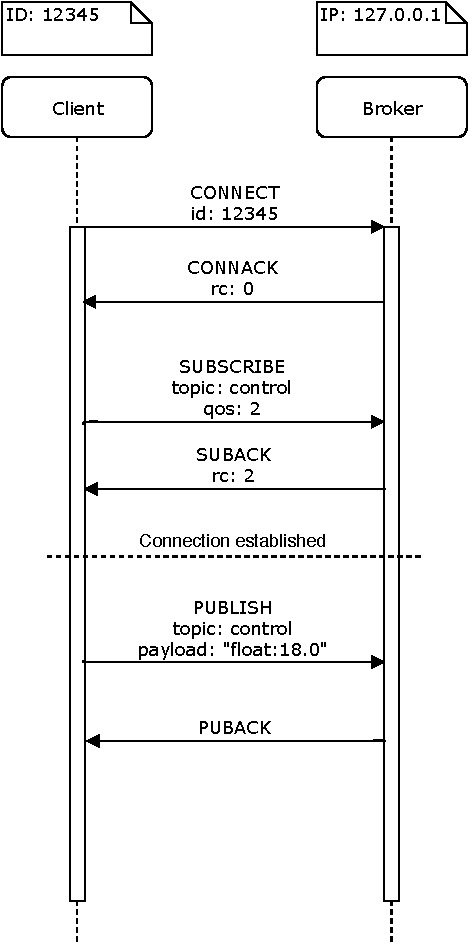
\includegraphics[width=0.5\textwidth]{obrazky-figures/MQTT-flow.pdf}
  \caption{Ukázka komunikace Klientu a Brokeru.}
  \label{mqtt-flow}
\end{figure}

\chapter{Implementace}
\label{sec:implementation}

\subsection{Knihovna $SNAKES$}

\href{https://www.ibisc.univ-evry.fr/~fpommereau/SNAKES/}{$SNAKES$} -- je knihovna v jazyce Python ktera nabizi vsechno potrebne pro definici a spousteni několíka variant Petriho sítí. Cilem knhovny $SNAKES$ je nabidnout badatelum moznost rychle namodelovat novy napad. Zvlastni vlastnosti knihovny $SNAKES$ je moznost vytvarzet Barevne Petriho site s pouzitim vyrazů v jazyce Python pro annotaci přechodu ci vstupnich nebo vystupnich šipek. \cite{snakes}

Zvlastni vlastnosti $SNAKES$ je moznost implementace vlastnich rozsireni pro jednotlive casti Petriho sítí, nebo pridani novych vlastnosti pro modelovani jinych podtypu Petriho sítí. Tato vlastnost byla zvlast pouzita v této prací pro pridani rozsireni, podporujici vytvareni Petriho sítí urcenych pro modelovani distribuovanych systému.
Jednou z nejdůležitějších pluginu je plugin umoznující přípojení \hyperref[sec:aplikace-mqtt]{MQTT clientů} pro provazani portu Petriho sítí mezi sebou.

\subsection{Implementace MQTT}
\label{subsec:mqtt_impl}
Pro implementací mqtt klientu v simulatoru byla použitá knihovna \href{https://pypi.org/project/paho-mqtt/}{\texttt{paho-mqtt}}. Tato knihovna obsahuje všechno potřebné pro nastavení komunikačních kanálů mezí porty vzdalených Petriho sítí. Na základě použití této knihovny konečný uživatel může nastavit zvolené místo v Petriho sítí jako vstupní nebo vystupní port. viz \ref{code:remote-in-out}. Jejích vzhled je nasledující:
\begin{figure}[hbt]
  \centering
  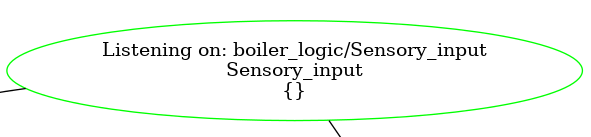
\includegraphics[width=0.5\textwidth]{obrazky-figures/port-in.png}
  \caption{Příklad vstupního portu}
  \label{port-in}
\end{figure}

\begin{figure}[hbt]
  \centering
  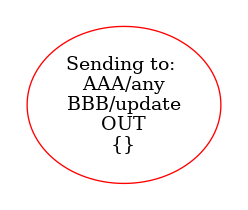
\includegraphics[width=0.5\textwidth]{obrazky-figures/port-out.png}
  \caption{Příklad výstupního portu}
  \label{port-out}
\end{figure}

Jak si můžete povšimnout, na rozdíl od ostatních míst sítě, vstupní a výstupní porty se označují barvou a dodatečným popisem. Pro vstupní port \ref{port-in} je to \texttt{Listening on: NET/TOPIC} a zelení barva, \texttt{Sending to: NET/TOPIC} pro výstupní \ref{port-out}. Ten, ve své řáde je označen červeně.

Je předem definované, že každá simulační instance odebírá zprávy z tématu \texttt{control}. Je to ekvivalent broadcastové adresy u IP.

Implementace zevnítř vypadá podobně reprezentací samotných portů. Sít, pří volaní metody \texttt{add\_remote\_input} nastaví týp místa na vstupní, pak pošle zprávu na téma \texttt{control} obsahující dvojicí [jméno sítě, jméno místa], a uloží zprávu do čekací fronty. Pak, když se k brokeru přípojí nějaká simulační instance s požadovanou dvojící síť--místo, tak se to oznamí všem ostatním simulačním instancím. To se zase provede zasilaním zprávy na téma \texttt{control}. Hned po příjetí takové zprávy se port nastaví a bude vykonavat svou čínnost.

\subsubsection{Směřování}
Na jeden vstupní port může být přípojeno 0 až několík vystupních portů, nebo jinymí slovy vstupní port příjma všechny zprávy na svoje temá.

\begin{figure}[htb]
  \begin{center}
    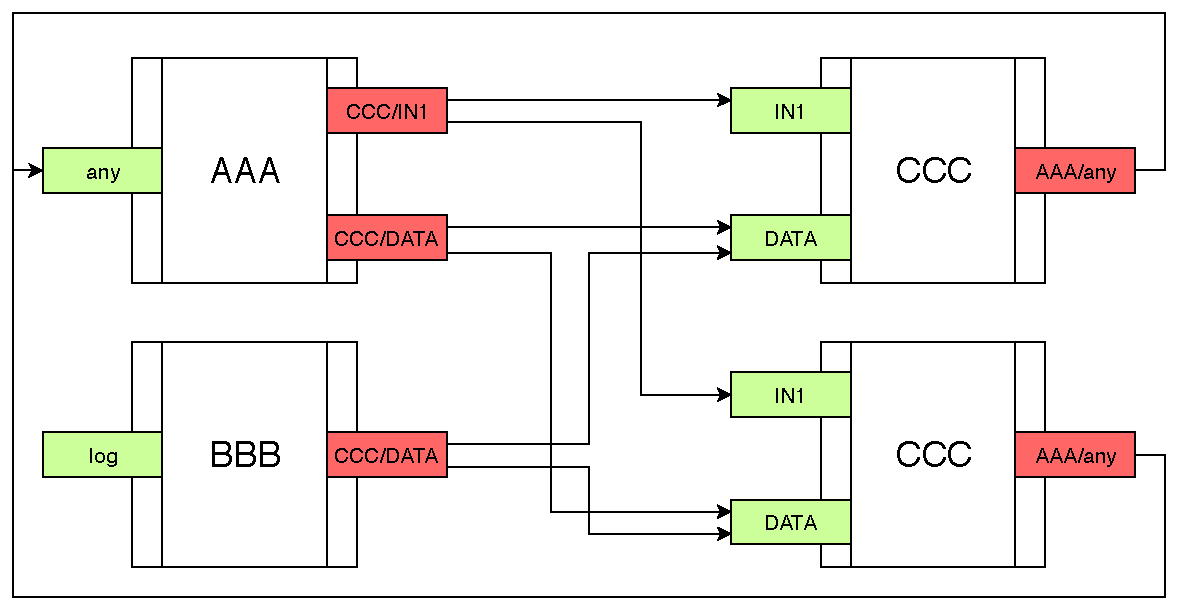
\includegraphics[width=0.7\textwidth]{obrazky-figures/Port-routing.pdf}
    \caption{Úkazka směřovaní zpráv.}
    \label{route-viz}
  \end{center}
\end{figure}

Na danem výše obrázku \ref{route-viz} můžete vidět ukázku směřovaní zpráv mezí porty. \texttt{AAA}, \texttt{BBB} a \texttt{CCC} jsou identifikatory Petriho sítí v ramcí jedného brokeru. Ve případě že se dvojice síť--port se vyskituje vícekrát, zprávy se přeposilají všem instancím. To si můžete všimnout na příkladu sítě \texttt{CCC}, která je na obrázku \ref{route-viz} dvakrát.

Na obrázku jsou 6 vstupních portů a 5 výstupních. Vstupní porty jsou označené zeleně, výstupní červeně. Jak je vidět na příklade dvoujic \texttt{CCC/IN1} a \texttt{CCC/DATA}, dvoující nemusí být unikatní. Počet přípojených výstupních portu k jednému vstupnímu není nějak omezen. Je to dosažene použítím vlastností MQTT klientu popsané v \ref{par:topic}.

Na příkladě vstupního portu \texttt{log} můžete vidět že není povinné, aby ten port byl zapojený. Ve případě simulatoru takový port nebude přiřázen do zkupíny vstupních portů, dokud se neobjeví nějaka applikace nebo síť, požadující přijetí a odesílaní zpráv na téma, kterou ten port odebírá. Více se o takovém nastavení viz \todo{ADD}

\subsection{Vlastní protokol komunikace}
Proto aby simulator měl podporu přídání vzdalených portů, zmíněnych v \ref{subsec:mqtt_impl} vznikla potřeba vymyslet vlastní protokol výměny informací. Ten protokol musí mít seznám zpráv pro takové simulační případy, kdy port musí předat nebo příjmout tokeny, nebo když se objeví instance Petriho síti v nějakém z už existujících či nově vytvořených simulačních úzlu. \todo{návod pro vytvoření takového}.

Nasledující tabulka \ref{tab:mqtt-msg-types} obsahuje přehled typů zpráv, a jejích formatu pro naplnění:

\begin{table}[H]
	\vskip6pt
	\caption{Tabulka typů zpráv}
    \vskip6pt
	\centering
	\begin{tabular}{llllr}
		\toprule
		Typ & Zkrátka & Formát \\
    \midrule
    Update & U & U\_ACTION, SRC\_SIM\_ID, NEW\_NET\_NAME \\
    Request & R & R\_ACTION, TARG\_NET/TARG\_PLACE, SRC\_NET/SRC\_PLACE \\
    Success & S & REQUEST\_COPY \\
    Failure & F & REQUEST\_COPY \\
		\bottomrule
	\end{tabular}
	\label{tab:mqtt-msg-types}
\end{table}

\paragraph{Update} Zprávy tohoto typu oznamují instancím simulatoru, jestli se v jejích okolí neobjevila nová Petriho síť, nebo naslouchající aplikace. Ve případě dodaní zprávy typu \uv{Update}, každá síť bude muset aktualizovat seznám svých aktivních portu, a ve případě že nějaký port čeká na nastavení, tak poslát požadavky na pro nově příchozího klienta. Poslední akcí je aktualizace tabulky znamých sití nově příchozího klienta, ve případě že klient není externí aplikace. Pro aplikaci je ten krok vynechan.
\todo{priklady}

\paragraph{Request} Tento týp zpráv nastavuje vstupní a výstupní porty. Parametr \uv{\texttt{R\_ACTION}} může nabývat hodnoty \texttt{set\_input} pro nastavení cíloveho místa \uv{\texttt{TARG\_PLACE}} jako vstupní port pro síť \uv{\texttt{TARG\_NET}}. Parametr \uv{\texttt{SRC\_NET}} je v tom případě není potřeba, stačí uvěst rozdelovač.

Příklad: \texttt{R, set\_input, net1/port1, /}

Pro nastavení výstupního portu stačí nastavit parametr

\subsection{Implementace pluginů}
\label{sec:plug-impl}
Tento pododdil popisuje implementaci růyných pluginu pro knihovnu $SNAKES$, které zesnadnuji návrch Petriho sítí a její modelovaní. Každý z níže popsaných pluginu se da  použít v kodu po jejích importu podle tohoto \href{https://www.ibisc.univ-evry.fr/~fpommereau/SNAKES/first-steps-with-snakes.html}{návodu}.

\subsection{Návod pro import rozšíření}
Vzhledem k odlišnému postupu pří přídání rozšíření do SNAKES, pro import simulačního nástroje a dalších rozšíření ze skupíny, užívatel musí dodřet správné pořadí pri importu knihoven. Konvence probíhá nasledujícím způsobem.

\begin{lstlisting}[language=Python, escapeinside={(*}{*)}, numbers=right, label={code:plugin-setup}]
  from snakes.nets import *   # Site, mista, prechody... (*\label{code:snakes-all}*)
  from simul import PNSim     # Simulacni knihovna (*\label{code:pnsim}*)
  snakes.plugins.load( (*\label{code:sim-plugins}*)
    ["gv", "timed_pl", "sim_pl", "prob_pl", "prior_pl"],
    "snakes.nets",
    "plugins") # Seznam rozsireni pro import
  from plugins import * # Redefinovane metody z rozsireni (*\label{code:pl-import}*)
\end{lstlisting}

\begin{enumerate}
  \item Pridani knihovny snakes a její prvků \ref{code:snakes-all}.
  \item Import simulační knihovny, která poskytné základ pro pluginy \ref{code:pnsim}.
  \item Přidaní pluginů podle požadovaných vlastností síte \ref{code:sim-plugins}. Ze skupíny doporučených pluginů stojí za zmínku plugin \href{https://www.ibisc.univ-evry.fr/~fpommereau/SNAKES/API/plugins/gv.html}{\uv{gv}}. Více o jeho použítí v ramcí simulatoru viz. \todo{}. Zbýtek je popsán v dalších sekcích \ref{subsec:timed_pl}.
  \item Pro redefinici a přidání nových metod z rozšíření slouží řádek \ref{code:pl-import}. Od dané chvilí použítí knihovný SNAKES je stejné jako v \href{https://www.ibisc.univ-evry.fr/~fpommereau/SNAKES/first-steps-with-snakes.html}{návodu} a taky \todo{Muj navod}.
\end{enumerate}

\subsubsection{Plugin \texttt{timed\_pl}}
\label{subsec:timed_pl}
Toto rozsireni pouziva planovac udalosti pro spolehlive planovani spousteni tranzice do budoucna. Toto rozsireni pouziva jednoduchou logiku pro provedeni přechodu - ve chvili kdy přechod bude spustitelny, tak se zapne casovac a zkonzumuji odpovidajici tokeny ze vstupnich mist. Cekani se neresetuje pridanim dalsich tokenu do vstupnich mist. Ve pripade teto implementace přechod vezme noveprichozi tokeny ktere se objevi ve vstupnich mistech a tudiz zapnou tranzici. Po ukonceni cekani, tokeny budou preneseny do vystupnich mist, s nasledujcimi upravami, ktere můžou nastat podle definice HLPN(odkaz).
\begin{figure}[hbt]
  \centering
  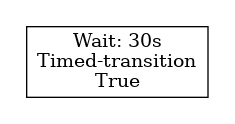
\includegraphics[width=0.3\textwidth]{obrazky-figures/timed-transition.png}
  \caption{Příklad časovaného přechodu}
  \label{timed-transition}
\end{figure}

\subsubsection{Plugin \texttt{prob\_pl}}
\label{subsec:prob_pl}
Toto rozsireni pridava moznost spojit nekolik tranzici do jedne skupiny, a tudiz rovnomerne rozdelit pravdepodobnost spousteni kazde z nich. Pro spojene přechody plati, ze museji mit stejnou sadu vstupnich mist. Pak se pri provedeni jedneho z nich se rozhodne na zaklade hodnoty jeho pravdepodobnosti jestli se tento přechod musi provest, nebo se provede nektery z jeho sousedu. Soucet pravdepodobnosti pro takovou skupinu přechodu musi byt vzdycky 1.
\begin{figure}[hbt]
  \centering
  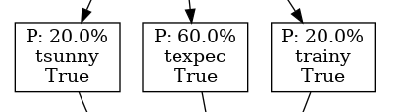
\includegraphics[width=0.6\textwidth]{obrazky-figures/prob-transition.png}
  \caption{Příklad pravděpodobnostního přechodu}
  \label{prob-transition}
\end{figure}

\subsubsection{Plugin \texttt{prior\_pl}}
\label{subsec:prior_pl}
Tento plugin je urceny pro pridani priorit k pechodum v siti. Podle nastavene priority se behem simulace bude rozhodovat, ktere tranzice se vyhodnoti a provedou jako prvni. Priority můžou byt v rozsahu 0 -- 100, a radi se sestupne. Pro nastaveni priority element `Transition` má dodatečný a nepovinný parametr `prior`. 
\begin{figure}[hbt]
  \centering
  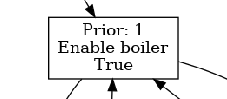
\includegraphics[width=0.3\textwidth]{obrazky-figures/prior-transition.png}
  \caption{Příklad prioritního přechodu s prioritou $1$}
  \label{prior-transition}
\end{figure}

\subsection{Plugin \texttt{sim\_pl}}
\label{sec:aplikace-mqtt}
Na implementací tohoto pluginu je založená práce ostatních pluginů ze skupiny \ref{sec:plug-impl}. Je ve své podstatě spojovacím prvkém mezi simulatorem, $MQTT$ klientem a sětí Petri. Obsahuje přetežovaní metod ze knihovny $SNAKES$ pro vykreslování prvků, které jsou rozšiřené pluginy. Taky přidavá zasadní metody pro nastavení Petriho sítě, umožnující použítí simulatoru a provadění spouštění sítě \ref{code:add_simulator}.
\begin{lstlisting}[language=Python, escapeinside={(*}{*)}, numbers=right]
  sim = PNSim()
  n = PetriNet('Sample net')
  n.add_simulator(sim) (*\label{code:add_simulator}*)
\end{lstlisting}

Stejně tak podporuje nastavení vzdalených portů pro předaní tokenů jiným sítím připojeným na stejnou adresu $MQTT$ brokeru \ref{code:remote_in}, \ref{code:remote_out}.

\begin{lstlisting}[language=Python, escapeinside={(*}{*)}, numbers=right, label={code:remote-in-out}]
  n.add_remote_input(it, 'temp_gen/Measurement') (*\label{code:remote_in}*)
  n.add_remote_output(hen, 'boiler_logic/Sensory_input') (*\label{code:remote_out}*)
\end{lstlisting}


\subsection{Planovac udalosti}
\url{https://docs.python.org/3/library/heapq.html}
Planovac udalosti je naimplementovan jako prioritni fronta za vyuziti vestavene knihovny heapq v Pythonu. Api naznacuje ze pro pridani a vyberu prvku se pouzivaji metody $heappush$ a $heappop$. \url{https://docs.python.org/3/library/heapq.html#theory} Priorita v takove fronte se urcuje ciselnou hodnotou, ktera se vklada do fronty. Tato hodnota muze byt prvnim prvkem v seznamu elementu. Druhym parametrem pro urceni priority je poradi, ve kterem prvek byl vlozen. Tato sada pravidel umoznuje vkladat zaznamy, obsahujici cas spusteni jako prvni prvek, a podle toho se zaradi na prisluhujici misto ve fronte. Metoda $heappop$ vybere prvek ze seznamu s nejvyssi prioritou, coz bude element s nejnizsi hodnotou casu.
\chapter{Aplikace}
\section{Tepelne rizeni}
Pro demonstraci praci simulatoru bylo rozhodnuto namodelovat dystribovany system modelujici chovani topení, ktey nekteri z vas pravdepodobne pouzivaji u sebe doma. Takovy system se sestavuje z nekolika casti. Zakladnim prvkem je plynovy spotrebic, nebo karma. Ta ohriva vodu a uvadi ji do pohybu po potrubich. Pak kazdy z pokoju ma na starosti ?teplene cidlo? a rizeni, ktere udrzuje v pokoji nastavenou teplotu podle calendare. Kazdou hodinu se z tabulky teplot vezme aktualni teplota pro soucasnou hodiny a tento pokoj, pak rizeni rozhodne jestli ma zapnout topení nebo ne. Pokud zadny z pokoju v soucasne dobe nema zapnute topení, tak karma se musi vypnout za ucelem setreni plynu. Toto rizeni provadi vestaveny system, nebo je zcela mechanicky. Kazdy z tech prvku bude dale namodelovan Petriho siťěmi.

Aby tento navrh co nejpresneji odpovidal realite, bylo rozhodnuto namodelovat chovani teploty v pokoji.
Nejdrive musime vedet jak vykonne je topení v pokoji. Běžné hodnoty pro tři druhy pokujů mužete videt v nasledujici \hyperref[tab:TepelneZtraty]{tabulce}. Dale nas zajimaji tepelné ztraty a taky mnozstvi energii potrebne pro ohrati pokoje. Pro vypocet tohoto parametru pouzijeme nasledující vzorecek. Zakladni parametrem rozhodujicim o tepelnych kapacite pokoje je plocha vnitrniho povrchu pokoje $V$, respektive celkova plocha povrchu stopu, podlahy a sten. Pro ně je dulezte vědět koefficent ztrat tepla $K$. Zvlast se pocitaji okna a dvere, vzhledem k jejich vetshi teplovodivosti. Pak zbyva jenom zjistit rozdil současné teploty uvnitr pokoje a očekavane teploty pro tuto hodínu - $\Delta{T}$. To vsechno dosadime do vzorecku a zjistime celkové mnozstvi energii potrebne pro jeho ohrati. \cite{tep_calc}
\begin{center}
  $Q[kW/h] = \frac{V*\Delta{T}*K}{860}$
\end{center}

Pro zjednoduseni vypoctu zanedbame parametry koefficentu ztrat tepla pro vsechny elementy, a vezmeme stredni hodnoty pro nekolik typickych druhu pokoju - kuchin, sklep a obyvaci pokoj. Kazdy z techto pokoju bude mit odlisny koefficent K a V. Pokoj bude mit 2 steny celici venku, kuchin bude mit 1. Pro sklep navic plati konstantni teplota vnejsiho prostredi, napriklad 5 stupnu. Taky se budeme pocitat s prijemnymi (skoro tropickymi) podminkami Ceske republiki - teplota venku je v prumeru v rozmezi 5 az 10 stupnu. \cite{cesko}
Pak koefficenty vypadáji nasledně:

\begin{table}[H]
	\vskip6pt
	\caption{Tabulka parametrů pokojů}
    \vskip6pt
	\centering
	\begin{tabular}{lllr}
		\toprule
		Typ pokoje & Koefficent tepelných ztrat & Objem $[m^3]$ & Očekavaný výkon topení $[W]$ \\
    \midrule
    Kuchin & 0.5 & $4*3*2.5$ & $1200$ \\
    Pokoj & 0.6 & $6*4*2.5$ & $2300$ \\
    Sklep & 0.8 & $3*3*2.2$ & $300$ \\
		\bottomrule
	\end{tabular}
	\label{tab:Parametry}
\end{table}

Na vypocet tepelnych ztrat pokoje jsem pouzil tento nastroj. \url{https://wpcalc.com/kalkulyator-teplopoter/}
Vychazí to zhruba nasledne:

\begin{table}[H]
	\vskip6pt
	\caption{Tabulka tepelných ztrát pokojů}
    \vskip6pt
	\centering
	\begin{tabular}{llr}
		\toprule
		Typ pokoje & Ztráty $[kW/h]$ \\
		\midrule
		Kuchin & $0.7$ \\
    Pokoj & $1$ \\
    Sklep & $0.4$ \\
		\bottomrule
	\end{tabular}
	\label{tab:TepelneZtraty}
\end{table}

Cele chovani systému odpovida zákonu zachovaní energii, a tak muzeme odvodit rovnici pro vypocet potrebneho jeji mnozstvi.


Modelovani chovani teploty venku je stochasticky process, ktery neni mozne spocitat presne. Proto byla navyrzena Petriho sit, vyuzivajici pravděpodobnostní přechody. Ma na vstupu rozsah teplot den - noc, a podle vybrane doby dne, za pouziti funkcii $cos$ modeluje zmenu aktualni teploty. Rozhodnuti pouziti funkce $cos$ vychazi z jednoducheho pozorovani prubehu teplot behem dne, a pereodicita zmeny teplot ji trochu odpovida, za predpokladu ze prubeh funkce zacina v nejteplejsi hodinu. %https://forecast.weather.gov/MapClick.php?lat=42.3758&lon=-71.1187&lg=english&FcstType=graphical
Pravděpodobnostní přechody modeluji nahodne jevy jako oteplení nebo ochlazení kvůli východu sluncie nebo jiné.


\chapter{Závěr}
\label{zaver}
